%
% This is the VPH 2016 mini paper.
%
% It's an example of using latex for a paper of specified size/layout.
%

% While writing, don't stop for errors
\nonstopmode

% Use the article doc class, with an 11 pt basic font size
\documentclass[11pt, a4paper]{article}

% Makes the main font Nimbus Roman, a Times New Roman lookalike:
%\usepackage{mathptmx}% http://ctan.org/pkg/mathptmx
% OR use this for proper Times New Roman (from msttcorefonts package
% on Ubuntu). Use xelatex instead of pdflatex to compile:
\usepackage{fontspec}
\usepackage{xltxtra}
\usepackage{xunicode}
\defaultfontfeatures{Scale=MatchLowercase,Mapping=tex-text}
\setmainfont{Times New Roman}

% Set margins to match VPH layout
\usepackage[margin=2.5cm]{geometry}

% Multilingual support
\usepackage[english]{babel}

% Nice mathematics
\usepackage{amsmath}

% Control over maketitle
\usepackage{titling}

% Section styling
\usepackage{titlesec}

% Ability to use colour in text
\usepackage[usenames]{color}

% For the \degree symbol
\usepackage{gensymb}

% Allow includegraphics and nice wrapped figures
\usepackage{graphicx}
\usepackage{wrapfig}
\usepackage[outercaption]{sidecap}

% Set formats using titlesec
\titleformat*{\section}{\bfseries\rmfamily}
\titleformat*{\subsection}{\bfseries\itshape\rmfamily}

% thetitle is the number of the section. This sets the distance from
% the number to the section text.
\titlelabel{\thetitle.\hskip0.3em\relax}

% Set title spacing with titlesec, too.  The first {1.0ex plus .2ex
% minus .7ex} sets the spacing above the section title. The second
% {-1.0ex plus 0.2ex} sets the spacing the section title to the
% paragraph.
\titlespacing{\section}{0pc}{1.0ex plus .2ex minus .7ex}{-1.1ex plus 0.2ex}

%% Trick to define a language alias and permit language = {en} in the .bib file.
% From: http://tex.stackexchange.com/questions/199254/babel-define-language-synonym
\usepackage{letltxmacro}
\LetLtxMacro{\ORIGselectlanguage}{\selectlanguage}
\makeatletter
\DeclareRobustCommand{\selectlanguage}[1]{%
  \@ifundefined{alias@\string#1}
    {\ORIGselectlanguage{#1}}
    {\begingroup\edef\x{\endgroup
       \noexpand\ORIGselectlanguage{\@nameuse{alias@#1}}}\x}%
}
\newcommand{\definelanguagealias}[2]{%
  \@namedef{alias@#1}{#2}%
}
\makeatother
\definelanguagealias{en}{english}
\definelanguagealias{eng}{english}
%% End language alias trick

%% Some aliases
\newcommand{\ccg}{Cope-Chambers-Prescott-Gurney}
\newcommand{\brain}{brain}
\newcommand{\stob}{S2B}
% Emphasis and bold.
\newcommand{\e}{\emph}
\newcommand{\mycite}[1]{\cite{#1}}
%% END aliases

% VPH font defs
% fontsize is \fontsize{fontsize}{linespacesize}
\def\authorListFont{\fontsize{11}{11} }
\def\corrAuthorFont{\fontsize{10}{10} }
\def\affiliationListFont{\fontsize{11}{11}\itshape }
\def\titleFont{\fontsize{14}{11} \bfseries }
\def\textFont{\fontsize{11}{11} }
\def\sectionHdrFont{\fontsize{11}{11}\bfseries}
\def\bibFont{\fontsize{10}{10} }
\def\captionFont{\fontsize{10}{10} }

% Caption font size to be small.
\usepackage[font=small,labelfont=bf]{caption}

\def\firstAuthorLast{James {et~al.}}

% Affiliations
\def\Address{\\
\affiliationListFont 1 Adaptive Behaviour Research Group, Department of Psychology,
  The University of Sheffield, Sheffield, UK \\
\affiliationListFont 2 Insigneo Institute for in-silico Medicine,
  The University of Sheffield, Sheffield, UK \\
\affiliationListFont 3 Department of Computer Science,
  The University of Sheffield, Sheffield, UK \\
\affiliationListFont 4 Department of Automatic Control Systems Engineering,
  The University of Sheffield, Sheffield, UK \\
\affiliationListFont 5 Department of Computer Science,
  The University of Patras, Patras, Greece \\
}

% The Corresponding Author should be marked with an asterisk. Provide
% the exact contact address (this time including street name and city
% zip code) and email of the corresponding author
\def\corrAuthor{Kevin Gurney}
\def\corrAddress{Department of Psychology, The University of Sheffield,
  Western Bank, Sheffield, S10 2TP, UK}
\def\corrEmail{k.gurney@sheffield.ac.uk}

% Figure out the font for the author list..
\def\Authors{\authorListFont Sebastian James\,$^{1,2}$, Alexander Blenkinsop\,$^{1,2}$,
  Alexander Cope\,$^3$, Sean Anderson\,$^{2,4}$, \\
  \authorListFont Chris Papapavlou\,$^5$, Konstantinos Moustakas\,$^5$, Kevin
  Gurney\,$^{1,2,*}$ \\[1 ex]  \Address \\
  \corrAuthorFont $^{*}$ Correspondence: \corrEmail}

% No page numbering please
\pagenumbering{gobble}

% A trick to get the bibliography to show up with 1. 2. etc in place
% of [1], [2] etc.:
\makeatletter
\renewcommand\@biblabel[1]{#1.}
\makeatother

% reduce separation between bibliography items if not using natbib:
\let\OLDthebibliography\thebibliography
\renewcommand\thebibliography[1]{
  \OLDthebibliography{#1}
  \setlength{\parskip}{0pt}
  \setlength{\itemsep}{0pt plus 0.3ex}
}

% Set correct font for bibliography (doesn't work yet)
%\renewcommand*{\bibfont}{\bibFont}

% No paragraph indenting to match the VPH format
\setlength{\parindent}{0pt}

% Skip a line after paragraphs
\setlength{\parskip}{0.5\baselineskip}
\onecolumn

% titling definitions
\pretitle{\begin{center}\titleFont}
\posttitle{\par\end{center}\vskip 0em}
\preauthor{ % Fonts are set within \Authors
        \vspace{-1.1cm} % Bring authors up towards title
        \begin{center}
        \begin{tabular}[t]{c}
}
\postauthor{\end{tabular}\par\end{center}}

% Define title, empty date and authors
\title {
  Integrating brain and biomechanics for the study of
  Parkinson's disease
}
\date{} % No date please
\author{\Authors}

%% END OF PREAMBLE

\begin{document}

\setlength{\droptitle}{-1.8cm} % move the title up a suitable amount
\maketitle

\vspace{-1.8cm} % HACK bring the introduction up towards the title. It
                % would be better to do this with titling in \maketitle

\section{Introduction}

\begin{wrapfigure}{r}{0.4\textwidth}
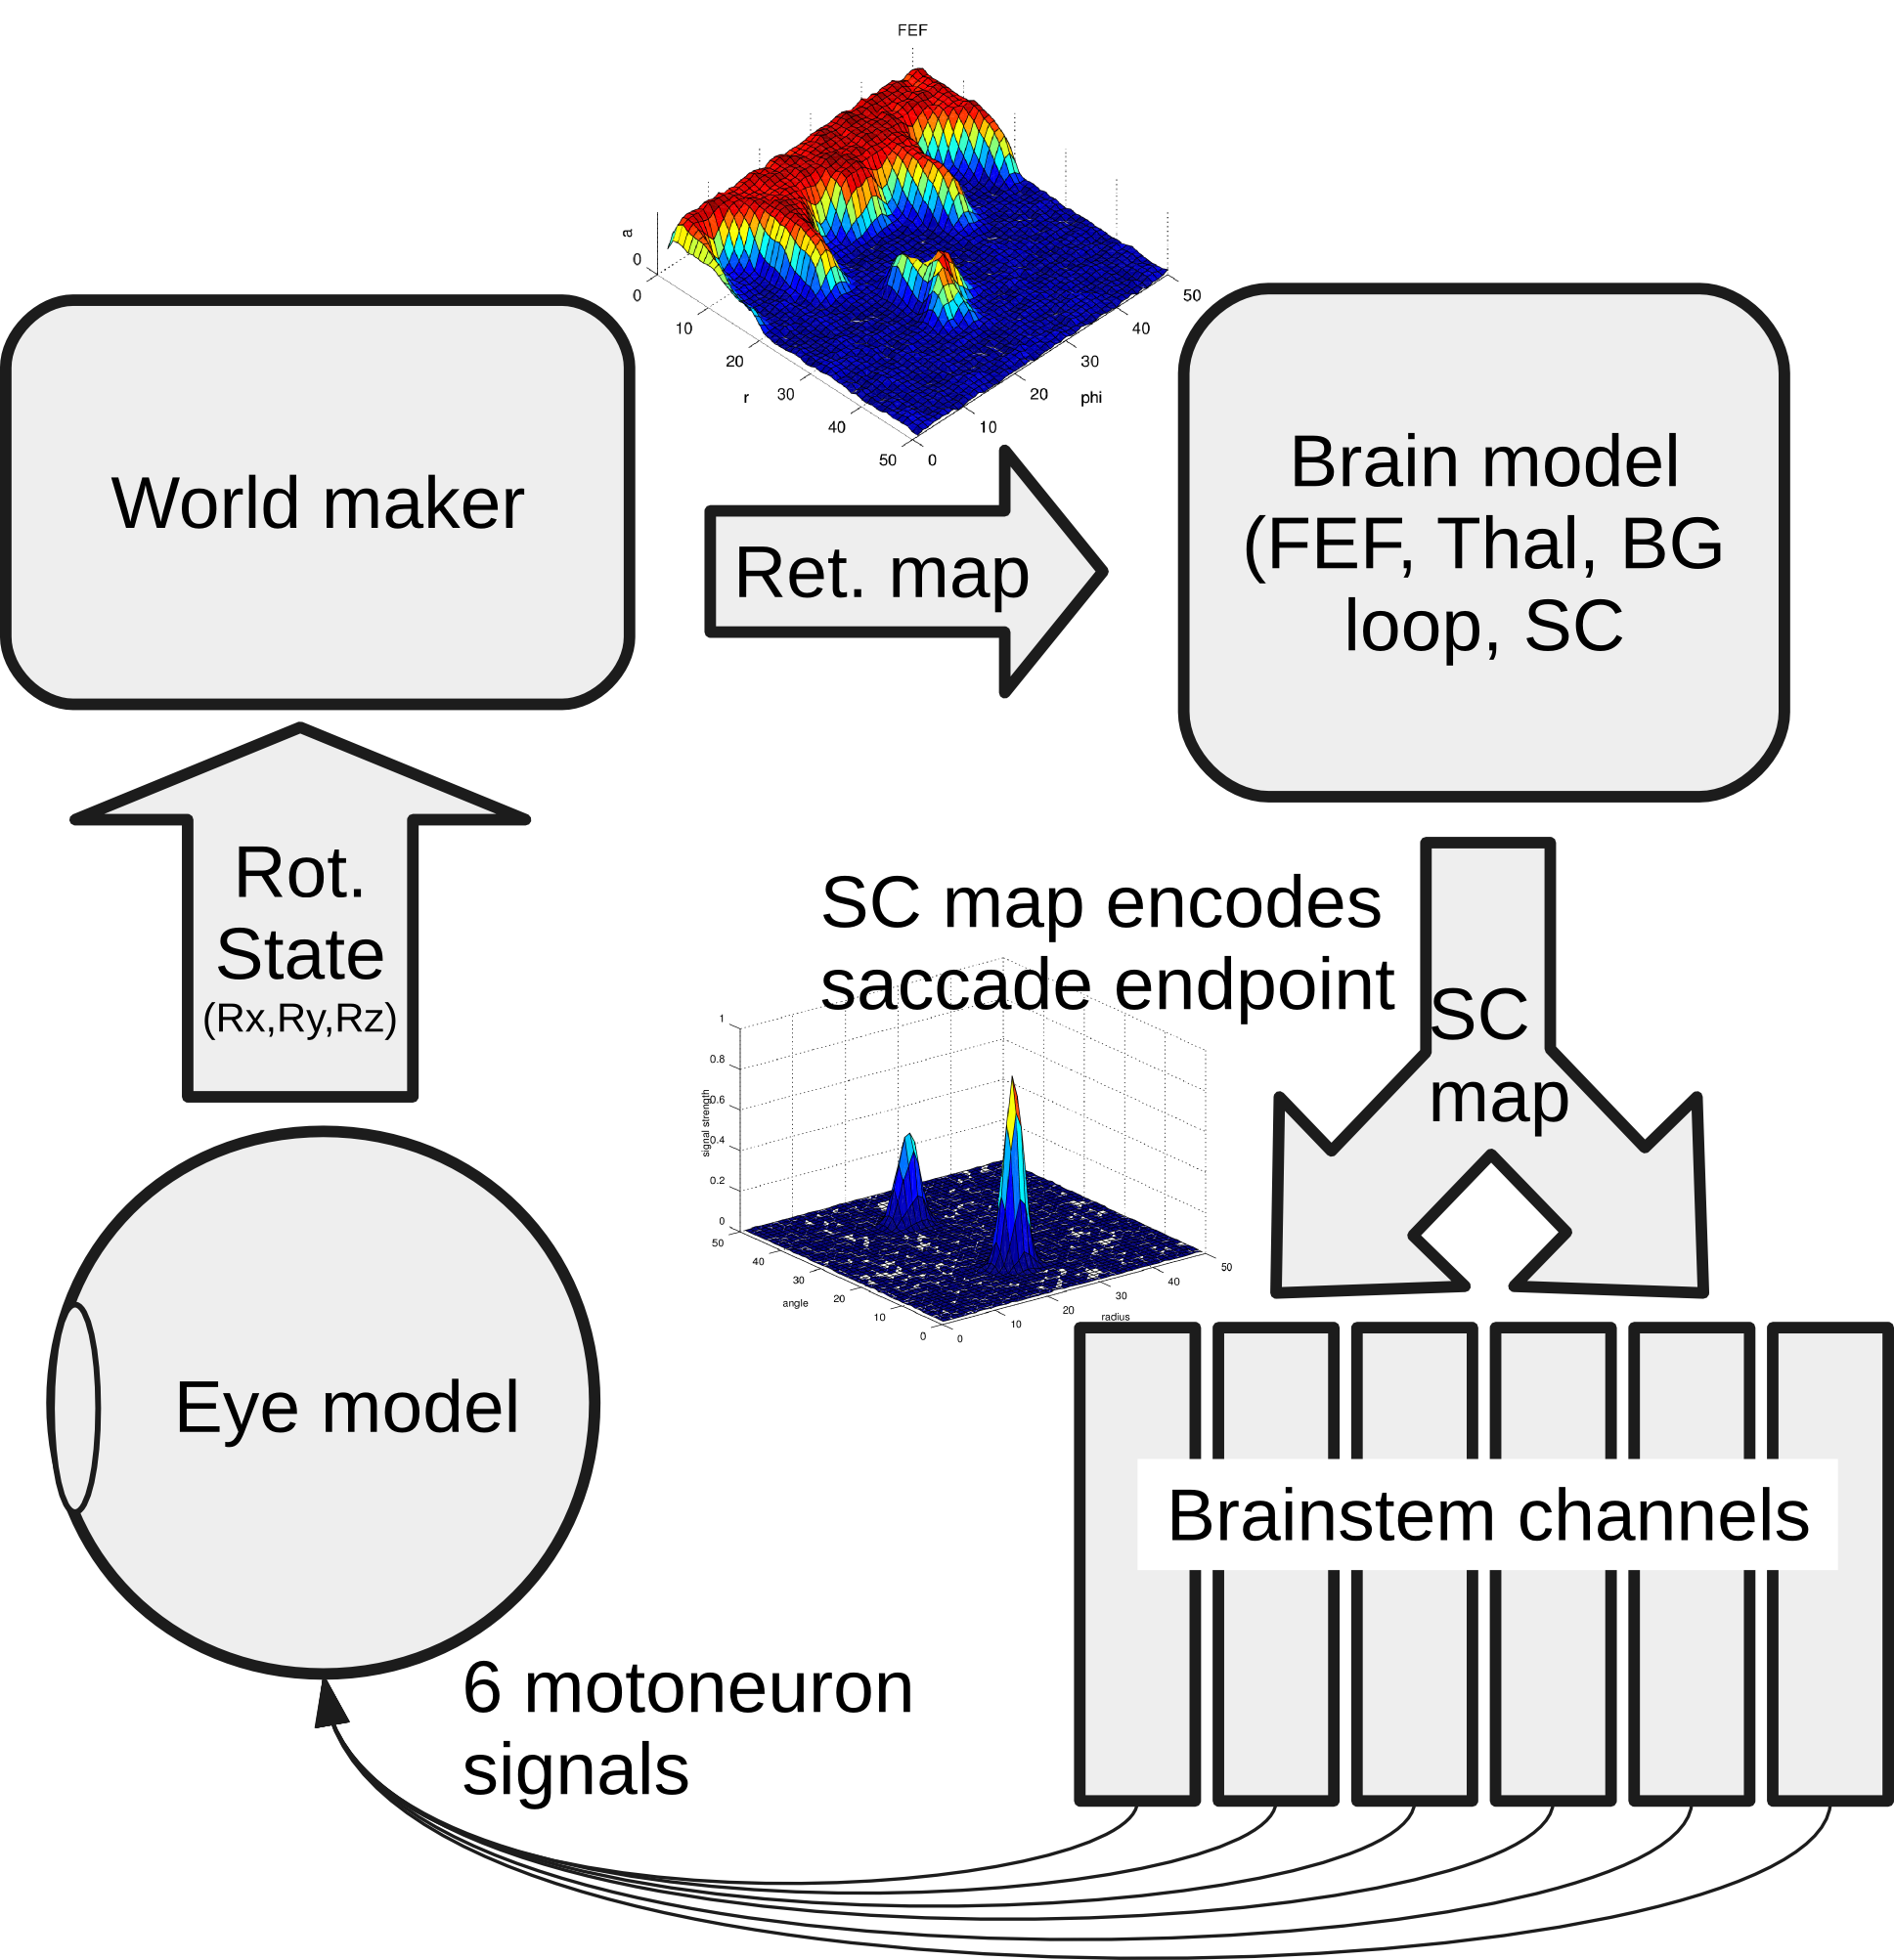
\includegraphics[width=0.4\textwidth]{./figures/model_overview.png}
\caption{The integrated model. The World maker component combines a
pre-defined series of luminances and the eye's rotational state to
produce a retinotopic map of the world in the eye's frame of reference
(an example surface map is shown for two cross-shaped luminances; one
at the fovea and one in the periphery). This is passed into
the \brain~model, which consists of retinal, cortical, basal ganglia
and collicular populations. The output of the \brain~model is encoded
as activity in a superior colliculus population (an example surface
map is shown for two peripheral luminances). Three pairs of brainstem
channels convert this position-encoded information into 6
time-dependent motoneuron signals which drive the eye model, updating
its rotational state.}
\vspace{-10pt}
\label{model_overview}
\end{wrapfigure}

% Can make comparisons
As mechanistic computational models of brain systems become more
sophisticated we can aspire to make realistic comparisons between the
behaviour of the model and that of the animal or human. This motivates
the development of \e{integrated brain and biomechanical systems}, to
express behaviour either in a virtual musculature or in an embodied
robotic system.

% Sometimes, ok to just have a brain model
In some cases, it is sufficient to take the activity of a neural
population as being representative of induced behaviour in the
individual. For example, a choice made in a \e{go/no-go} task could be
determined from activity in a population within a basal ganglia model
\mycite{nambu_discharge_1990,kuhn_event-related_2004}. The decision
to \e{go} is selected by a reduction of activity in this population;
maintenance of activity implies \e{no-go}. Error rates in this task
could be compared with experimentally determined error rates in
primate subjects, validating the model for the healthy subject.
% Now describe comparison between model and expt. for diseased
% subject.
If we can identify a characteristic degradation in the brain of an
unhealthy subject, then we can modify suitable parameters in the model
to reproduce it. By comparing the relationship between the model's
behaviour as a function of the degradation parameters with the
unhealthy individual's behaviour as a function of disease progression,
we may be able to relate the disease progression to the brain state
and predict the time-course of internal changes in the brain.
% Leave further discussion along these lines to the discussion
% section.

% But sometimes you might need brain and neuromuscular model
Of course, many behaviours are more complex than a two-way
decision. In the disease state, it may be the \e{dynamics} of the
movement which progress with time, rather than any movement outcome or
error rate. A diagnostic task may produce movement characteristics
which correlate with disease progression such as the slow, jerky or
inaccurate movements seen in Parkinson's Disease. In order to
determine the validity of a model which describes more complex
movements, it is necessary to express the movement commanded by the
brain network as a realistic, simulated motion by means of a
biomechanical model.

% Say what we've done here, in short form.
Parkinson's Disease (PD) is a progressive neurological disorder whose
main symptoms relate to motor control. These include resting tremor,
slowness of movements (bradykinesia), difficulty in initiating
movement (akinesia) and
rigidity \mycite{galvan_pathophysiology_2008}. It is considered to be
a disease of the basal ganglia because during its progression,
dopamine producing neurons in the substantia nigra pars compacta die
away, affecting the striatum, which depends on endogenous dopamine for
correct operation \mycite{javoy-agid_is_1980}. The basal ganglia plays
an important role in decision making and action
selection \mycite{schultz_reward_2000}, including the selection of
saccadic eye movements
\mycite{hikosaka_role_2000} which direct gaze towards putative targets
of interest. In the later stages of Parkinson's Disease, changes in
eye movement dynamics are observed; patients show more latent saccades
to targets of interest \mycite{chambers_response_2010}. They also
exhibit poorer performance \mycite{kitagawa_relationship_1994} in the
so-called anti-saccade protocol \mycite{munoz_look_2004}, in which the
subject is instructed to make a saccade \e{away} from a visual
target. These progressive changes in saccade dynamics in PD provided
the motivation to develop an integrated brain and biomechanical model
of the saccadic system.

%Parkinson's Disease patients make significantly more
%errors; they will saccade \e{to} the visual target rather
%than \e{away} from it more often than healthy control subjects.

% Motivation here is to study movement disorders by means of a
% comparison between healthy subjects, the healthy model and diseased
% subjects and the diseased model.
%To study PD, we chose to express saccadic eye movements in an
%integrated model.

%\pagebreak

\section{Material \& Methods}

% Add one weight map figure
\begin{wrapfigure}{r}{0.4\textwidth}
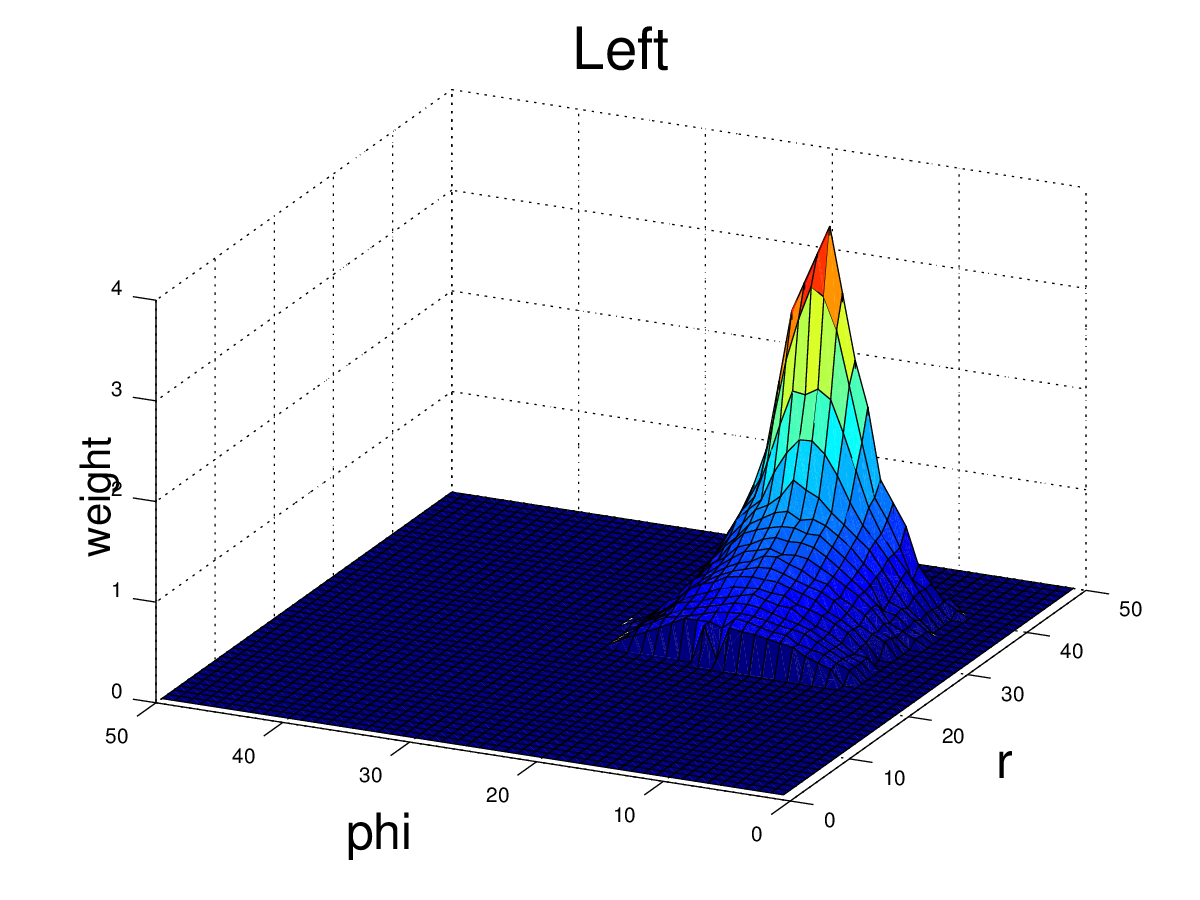
\includegraphics[width=0.4\textwidth]{./figures/w50_L.png}
\caption{One of six weight maps. This map makes a transformation from
a rotational position encoded in retinotopic space, where $r$ is
radial eccentricity and phi ($\phi$) is directional angle, extracting
the `leftwards rotation' component. For the left eye, this becomes
the command signal fed into the lateral rectus muscle. Note that $r$
and phi both have arbitrary units which scale from 1 to 50. These map
to $0\degree \leq \phi \leq 360\degree$ and $0\degree \leq r \leq
22\degree$.}
\vspace{-5pt}
\label{left_map}
\end{wrapfigure}

% A very short introduction to the section.
We started from the \ccg~model described
in \mycite{alex_cope_integrative_2015}, referred to here as
the \brain~model. This is a rate-coded neural network model
incorporating retinal populations, frontal eye fields (FEF), the basal
ganglia (BG), and the superior colliculus (SC). Rate-coded neural
elements are described by first order differential equations:
\[
   \dot{a} = {1 \over \tau}(a_{in}-a)
\]
where $\tau$ is the time constant for the neural activation and
$a_{in}$ is the input to the neural element. $a_{in}$ is defined by an
activation input and a shunting inhibition input according to: $a_{in}
= A(1-s_a)+0.01 R_N$. Here, $A$ is the activation input and $s_a$ is
the shunting inhibition state variable whose value is $S$ for $S\leq1$
and $1$ for $S>1$. $R_N$ is a random number between 0 and 1 drawn from
a normal distribution which introduces noise to the activation of the
neural element.

At each time step, the visual state of the `world' (as a retinotopic
map, with two axes $r$, radial eccentricity and $\phi$, directional
angle) is fed into the \brain~model, which then updates the state of
its output population, the SC (also a map). The `centre of mass' of
the activity in SC is assumed to accurately encode the location of the
eye at the end of the saccade \mycite{van_gisbergen_collicular_1987}.

To the \brain~model, we have added a saccadic burst generator (SBG)
model of neural populations in the brainstem's reticular formation,
which convert the position-encoding activity in the SC into motoneuron
signals \mycite{gancarz_neural_1998}, and a biomechanical eye
(Fig. \ref{model_overview}). The rotational state of the eye is used
to recalculate the view of the world in the eye's frame of reference
and then a retinotopic view is fed into back the \brain~model.

% short description of the brainstem model
The SBG is based on the model of two opposing channels described by
Gancarz and Grossberg in \mycite{gancarz_neural_1998}. This model
incorporates an internal inhibitory negative feedback loop and encodes
force in its output motoneurons. When integrating this model with
the \brain~model, it became clear that an inhibitory reset mechanism
was also required for the superior colliculus; without such a reset, a
series of staircase saccades would occur, as seen in SC stimulation
studies \mycite{schiller_single-unit_1972}. Recent evidence of
inhibitory retinotectal connections \mycite{wang_macaque_2010}
supports the inclusion of this connection in the model and makes
possible the removal of the internal negative feedback connection of
the Gancarz and Grossberg model, for which it is hard to find clear
evidence.

Input to the SBG comes from the SC of the \brain~model via
six retinotopic, many-to-one weight maps, an example of which is
shown in Fig.\ref{left_map}.

% EYE MODEL DESCRIPTION HERE
The biomechanical eye model, implemented using the OpenSim framework
\mycite{seth_opensim:_2011}, is anatomically represented by a sphere of
uniform mass distribution which is actuated by six extraocular muscles
(EOMs). The EOMs are arranged in three pairs forming a cone inside the
orbit with the apex being located inside the cranium in a tendonous
ring called the annulus of Zinn. An important feature of the
oculomotor system which greatly affects its overall behavior is the
existence of dynamic EOM pulleys. Their role is to guide the pivot
point of the EOMs. In our model, a pulley for each EOM has been
modeled by a point on the orbit whose location depends on the current
eye orientation.

%EOM dynamics
The force applied by EOMs is controlled by an excitatory signal
supplied by motoneurons in the brainstem. The dynamics of muscular
forces can be split into: 1) The elasticity of the muscles. 2) A delay
between the onset of the afferent excitatory signal and the actual
muscle contraction, caused by the transmission time of the action
potentials and by the necessary calcium release at the muscle
fibres. We developed a custom extraocular muscle model which captures
these features.
%Orbital fat force
Passive forces due to the fatty tissues inside the eye orbit also
affect eye dynamics. Their role is critical in eliminating the
influence of head and body movements. We incorporated a custom torque, $\mathbf{t}$,
which acts like a rotational spring-damper apparatus, resisting
eyeball movements. It has elastic and viscous properties governed by
$\mathbf{t} = -K\mathbf{R}-C\mathbf{U}$ where $\mathbf{R}$ is the
eye's orientation and $\mathbf{U}$ is its angular velocity. $K$ and
$C$ are constants.

% Say this one implemented in SpineML. (Could probably lose most of
% this)
The \brain~and SBG models were produced using SpineCreator
\mycite{cope_spinecreator_2015} and saved in the declarative,
simulator-agnostic markup language
SpineML \mycite{richmond_model_2014}. SpineML\_2\_BRAHMS
(\stob) \mycite{cope_spineml_2_brahms_2015-1} was used to simulate the
model.

%%%%%%%%%%%%%%% RESULTS FIGURE %%%%%%%%%%%%%%%%%%%%
% FIXME: add something about the fact that if the viscosity of the
% eye is too high, then saccades will be hypometric, or slow to
% arrive on target, underlining the need for an adaptive mechanism to
% tune the period during which the motoneuron output is at its
% ``high'' level.
%
% Figure is: Couple of rotation graphs. Taken from the model of branch
% 201605_VPH_2016_results with saccsim on branch
% brahms_201605_VPH_2016_results and SpineML_2_BRAHMS on branch
% NoTremor_Oculomotor_201603.
% Luminances file was:
% {"luminances":[
% {"shape":"cross","widthThetaX":6,"widthThetaY":2,"timeOn":0.15,"timeOff":10,
%  "thetaX":4,"thetaY":-8,"luminance":0.2}
% ]}
% OR:
% {"luminances":[
% {"shape":"cross","widthThetaX":6,"widthThetaY":2,"timeOn":0.15,"timeOff":10,
%  "thetaX":0,"thetaY":8,"luminance":0.2}
% ]}
%
\begin{wrapfigure}{R}{0.55\textwidth}
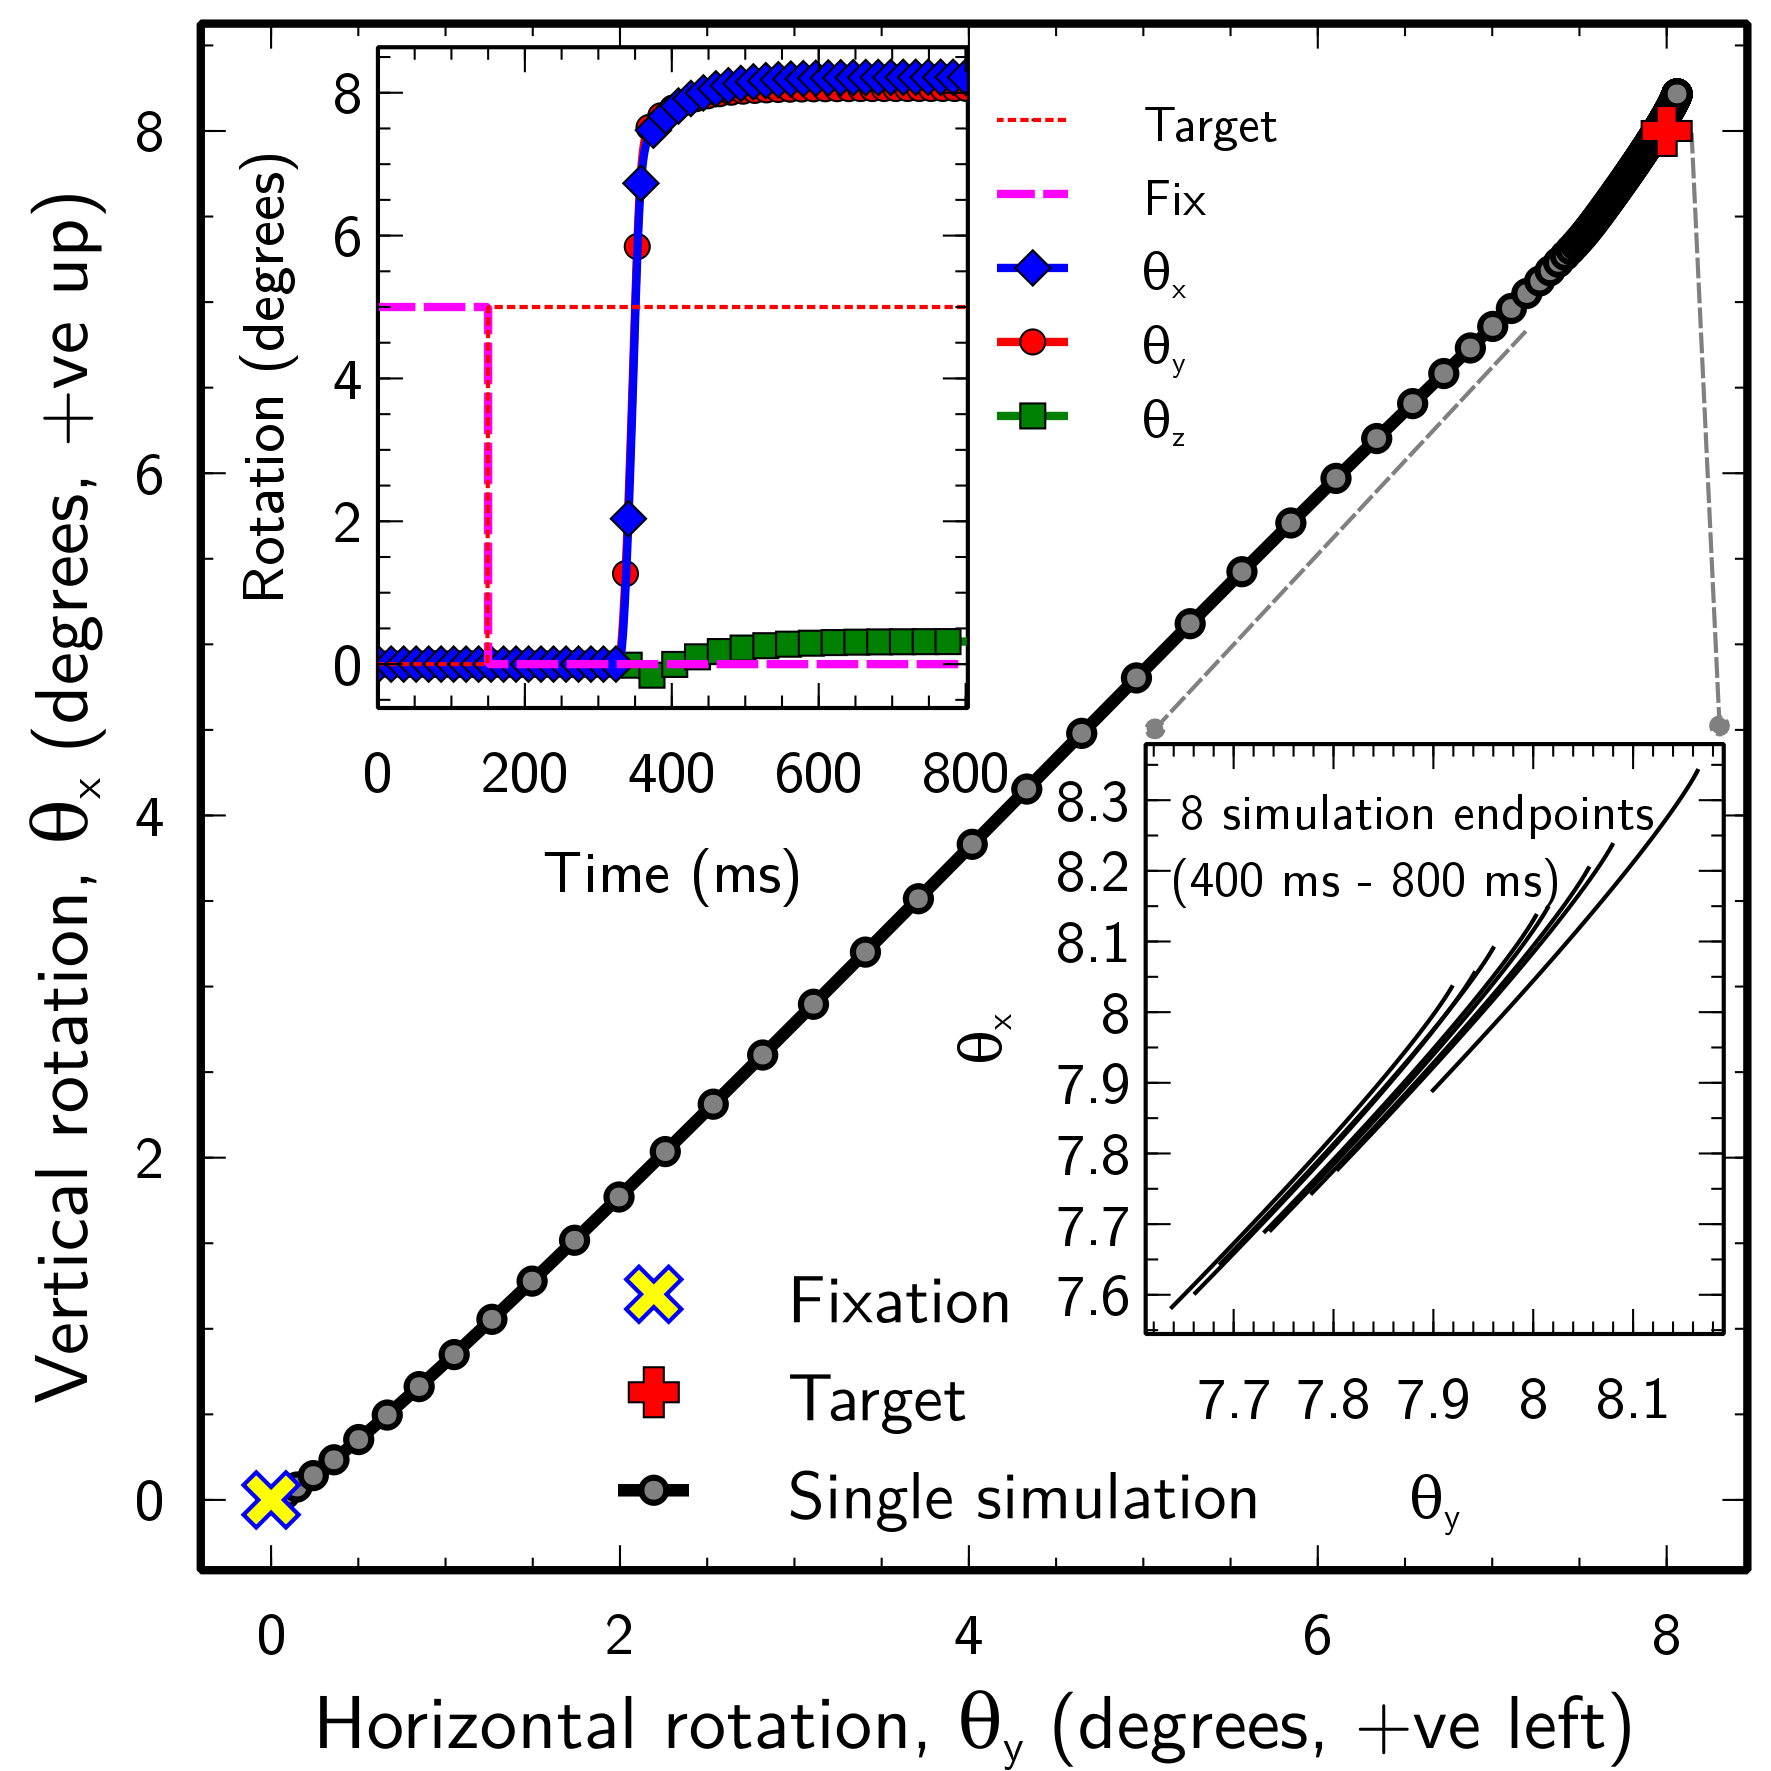
\includegraphics[width=0.55\textwidth]{./figures/results/20160523/vph_2016/trajectoryRX8RY8.png}
\caption{\textbf{Main graph:} Representative oblique saccade made by the
model from fixation to target locations shown. Data points are shown
at 1 ms intervals. \textbf{Top inset:} Three rotational components of
the trajectory plotted against time (a proportion of the data point
symbols have been omitted for clarity). Fixation and target luminance
positions are plotted as dashed and dotted lines. \textbf{Bottom
inset:} Endpoint scatter --- the latter part (400--800 ms) of 8
repeated simulations showing how noise in the \brain~model affects the
final rotation of the eye.}
\vspace{-10pt}
\label{trajectory}
\end{wrapfigure}
%%%%%%%%%%%%%%%%%%%%%%%%%%%%%%%%%%%%%%%%%%%%%%%%%%%

Three hand-written components are integrated into the
SpineML \brain~model: the biomechanical eye model; a component which
computes the centroid of a neural layer; and a component which takes
the eye's rotational state and the current visible luminances and
projects a retinotopic activity map into the \brain~model. Each of
these three BRAHMS components was hand written in C++.

% A description of the timestep issue
One challenge we encountered when integrating the eye model had to do
with the simulation time steps. The brain and brainstem models
required a common simulation time step of 1 ms, using a Forward Euler
solution method. The eye model worked optimally with a 25 ms time
step.  To resolve this issue, the eye model component was called on
each 1 ms timestep, but only recomputed its outputs every 25 time
steps.

% This section was previous under ``Results''
Parameters in the brain, brainstem and eye models were trained
independently. The \brain~model parameters were retained from
% well - unchanged apart from the dopamine params
\mycite{alex_cope_integrative_2015}. The brainstem model
was hand trained so that populations had temporal responses to match
experimental data from the literature. After integration, the six
weight maps between the superior colliculus and the SBG input neurons
were trained.
% How the model was trained, results of training.
%% Because there is noise in the \brain~model, a given luminance input
%% sequence does not always produce the same activity in superior
%% colliculus. As a result, it's not possible to record the activity
%% produced in SC for a given target luminance and then run a training
%% procedure which involves only the brainstem and eye model; the entire
%% model must be run for each iteration of the training process. This
%% makes the application of a traditional neural network training
%% algorithm, in which each weight map is regarded as a 2500-D weight
%% vector, computationally expensive.  To simplify the problem, the
%% centroid of the activity in the SC is computed, populating a map
%% called SC$_{avg}$. Only a single location in the SC$_{avg}$ map is
%% ever active, which means that for a given target luminance, it is
%% possible to write the same scalar weight in every element of the
%% weight map, which reduces the dimensionality of the weight space to
%% three.
Because there is noise in the \brain~model's output (See
Fig. \ref{trajectory}, lower inset), it is necessary to run the
entire, integrated model to train the SC to SBG weight maps. This
makes the application of a traditional neural network training
algorithm, in which each weight map is regarded as a 2500-D weight
vector, computationally expensive.
%It is not feasible to run the
%integrated model, which requires approximately two minutes on a
%typical CPU to simulate a single saccade, the many thousands of times
%required to find the solution in this high dimensional parameter
%space.
To simplify the problem, the centroid of the activity in the SC is
computed, populating a map called SC$_{avg}$. Only a \e{single
location} in the SC$_{avg}$ map is ever active, which means that for a
given target luminance, it is possible to write the same scalar weight
in all 2500 elements of the weight map, which reduces the
dimensionality of the weight space to three (one weight map for each
of three active extraocular muscles).  Input was given to the model in
the form of a target luminance at a given $(\theta_{x},\theta_{y})$
location. The weight maps were then adjusted in a gradient descent
process until the rotational angle of the eye after the first saccade
matched $(\theta_{x},\theta_{y})$, with $\theta_{z}=0$. The process
was repeated for a range of $(\theta_{x},\theta_{y})$.

%% Some detail omitted:
%The procedure makes the
%assumption that the components of the weight vector and the error
%vector are mutually orthogonal. This is not generally true, and so the
%weight training will not always complete; some target locations need
%to be re-run with differing start weights.

%Inspection of the weight maps shows that the weight increases
%approximately exponentially as a function of radial eccentricity, $r$,
%due to an exponential reduction in retinal neural density towards the
%edge of the field of view. A geometric argument would suggest that the
%weight should vary sinusoidally with the directional angle
%$\phi$ \mycite{tabareau_geometry_2007}.

\section{Results}

Our result for the shape of the weight maps (as in
Fig.~\ref{left_map}) agrees with theoretical work by Tabareau et
al. \mycite{tabareau_geometry_2007} and with a previous study which
computed weight maps in a similar
model \mycite{arai_two-dimensional_1994}. Additionally, our result
demonstrates that weight maps for the oblique muscles can be found
such that the axial rotation (R$_{ax}$) of the eye may follow a fixed
function of elevation (R$_{el}$) and azimuth (R$_{az}$); in this case
we required R$_{ax}$ = F(R$_{el}$,R$_{az}$) = 0 for all
R$_{el}$,R$_{az}$.

Fig.~\ref{trajectory} shows a resulting eye movement to a single
luminance target. A fixation (with luminance value 0.5) is presented
to the model for 150 ms. At 150 ms, the fixation is replaced by a
target at $\theta_{x}$=8$\degree$, $\theta_{y}$=8$\degree$ (a target
eye rotation of 8$\degree$~left and 8$\degree$~up). The saccade has a
realistic latency of 175 ms and a movement time of approximately 50
ms.

\section{Discussion and Conclusions}

% Be sure to say that ``in future work, it will be possible to
% investigate saccade trajectory modifications in Parkinson's''
We have demonstrated the integration of a \brain~model with a
neuromuscular model of three degrees of freedom. This model forms a
platform for the study of internal brain state in Parkinson's disease
and how this relates to saccade behaviour.
% Could lose this:
In future work it will be
possible to study saccade trajectory modifications with the
modification of dopamine expression in the model. It will be possible
to extend the model to examine antisaccade behaviour. It forms a
platform to study the effect of a more detailed treatment of portions
of the model, such as the incorporation of spiking models of basal
ganglia, a striatal microcircuit or a detailed simulation of the
superior colliculus.

\section*{Acknowledgements}
This work is partially funded by the EC FP7 project NoTremor --- Virtual,
Physiological and Computational Neuromuscular Models for the
Predictive Treatment of Parkinson's Disease, Grant Agreement
No.~610391.

\selectlanguage{English}
\bibliographystyle{abbrvnotitle}
% The bibliography NoTremor.bib is the one exported from Zotero.
\bibliography{NoTremor}

%%% Upload the *bib file along with the *tex file and PDF on
%%% submission if the bibliography is not in the main *tex file

\end{document}
